\section{Scheimpflug geometry}
\label{sec:scheimflug}
As introduced in the previous section, now, we describe the plane correction due to the application of Scheimpflug principle, tilting the lens. \\

Tilting lenses causes a variation of the image plane, which rotates to stay parallel to the lens itself. Many works, such as \cite{inproc-lens-inc}\cite{Louhichi2006}\cite{4059344}, tried to improve the calibration processes, introducing different corrections in order to balance the effects introduced by lens tilt. For the most part, they have tried to apply different rotations to the plane, but these have been shown to work only for small angles. For big angles, the rotations are not enough. \\

Consider the two image planes, the one parallel to the sensor and the tilted one: as shown in Figure \ref{fig:scheimpflug-line}, the origin of the two planes is the same, since the parallel plane can be arbitrarily placed.
  \begin{figure}[t!]
    \centering
    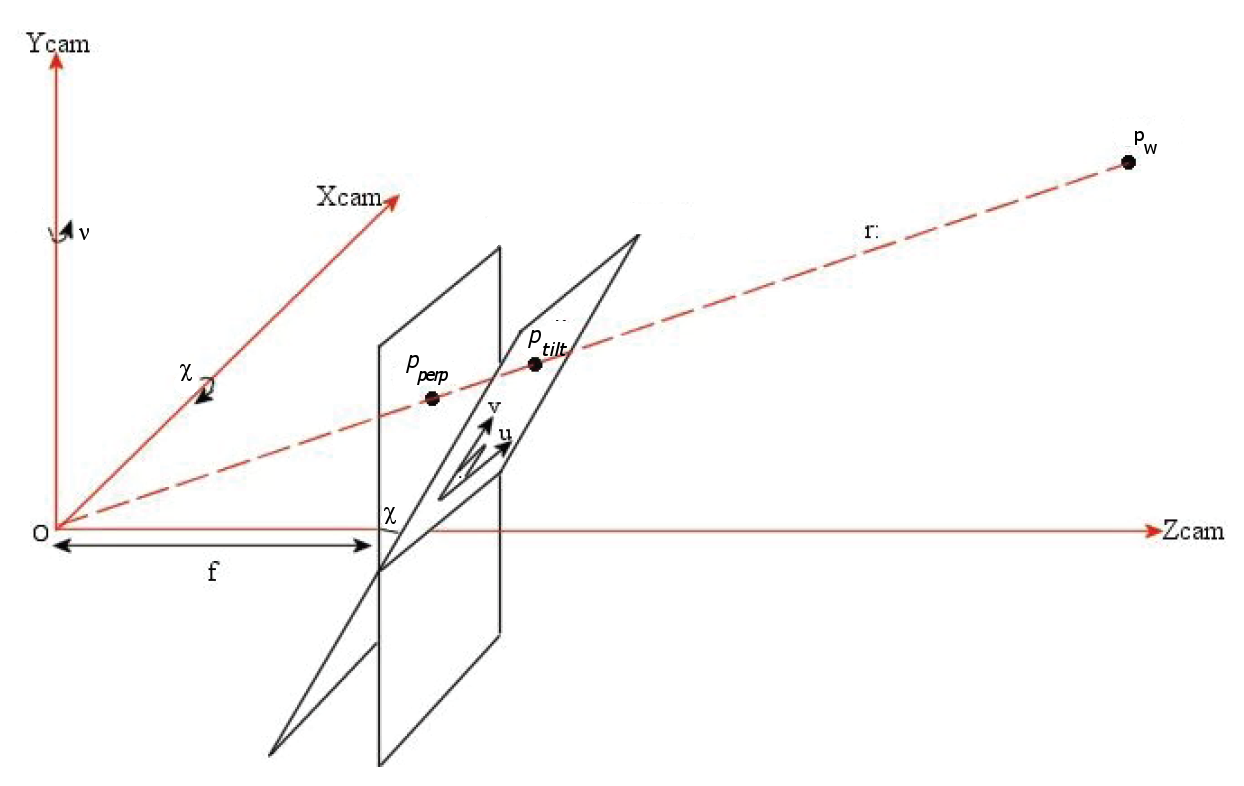
\includegraphics[width=\textwidth]{./images/model/scheimpflug.png}
    \caption{Intersection of the point in the real world in the tilted plane and in the perpendicular plane.}
    \label{fig:scheimpflug-line}
  \end{figure}
Similar to what is shown in the Figure \ref{fig:perspective_projection}, we can draw a line $r$ from the optical center $O$ to the point $p_w = \left( x_w, y_w, z_w \right)$ in the world. Accordingly with the sections above, $p_w$ is a point belonging to the laser plane, without considering radial compensation, and the tilted plane is the one in which we have projected $p_w$ in Section \ref{sec:wrd2cam}. Accordingly with \cite{SchCameraCalib}, the line $r$ passes through the two planes, allowing the definition of a system of equations that solve the intersection problem. The solution of this system can be written as follows:

  \begin{equation*}
      x_p = \lambda \cdot \left( x_s \cdot \cos\chi + y_s \cdot \sin\upsilon\cos\chi \right)
  \end{equation*}
  \begin{equation*}
    y_p = \lambda \cdot y_s \cdot \cos\upsilon
  \end{equation*}
where $\left( x_p, y_p\right) = p_{perp}$ in the figure, and $\left( x_s, y_s\right)$ ($p_{tilt}$ in figure) are the coordinate of the point in the sensor reference system, introduced in the section above. The parameter $\lambda$ is the plane coefficient and it is:
  \begin{equation*}
    \lambda = \frac{f}{f + x_s \sin\chi + y_s \sin\upsilon\cos\chi}
  \end{equation*}
The angles $\chi$ and $\upsilon$ are the swing and tilt angle of the lens, respectively. In literature, the term swing refers to a rotation with respect to the $x$ axis, while tilt refers to a rotation with respect to the $y$ axis. \\

The equation considered has been defined in a proposal for an algorithm for camera calibration. Despite that, the model capability to consider point projections gives to it a big advantage over simple rotations: the fact that we are able to consider also perspective distortions, as we have done in Section \ref{sec:pinhole_camera} for world to camera coordinate systems transformations. Note that also in this case, the $x$ coordinates are function of the $y$ ones. \\

From an analytical point of view, this is the most delicate step. The big number of elements to consider makes this calculation a big source of error. The error propagation model suggests to compute

  \begin{equation*}
    \sigma_{x_{s_i}} = \sqrt{
      \left( \frac{\partial x_{s_i}}{\partial y_{p_i}} \right)^2 \sigma_{y_{p_i}}^2 +
      \left( \frac{\partial x_{s_i}}{\partial x_{p_i}} \right)^2 \sigma_{x_{p_i}}^2 +
      \left( \frac{\partial x_{s_i}}{\partial \upsilon} \right)^2 \sigma_\upsilon^2 +
      \left( \frac{\partial x_{s_i}}{\partial \chi} \right)^2 \sigma_\chi^2
    }
  \end{equation*}
  \begin{equation*}
    \sigma_{y_{s_i}} = \sqrt{
      \left( \frac{\partial y_{s_i}}{\partial y_{p_i}} \right)^2 \sigma_{y_{p_i}}^2 +
      \left( \frac{\partial y_{s_i}}{\partial x_{p_i}} \right)^2 \sigma_{x_{p_i}}^2 +
      \left( \frac{\partial y_{s_i}}{\partial \upsilon} \right)^2 \sigma_\upsilon^2 +
      \left( \frac{\partial y_{s_i}}{\partial \chi} \right)^2 \sigma_\chi^2
    }
  \end{equation*} \\
  
\noindent
Even in this case we could ignore the contribution of the focal length, because it is a parameter estimated by the calibration process.\\

To complete this model, we should take into account also focal length and image center transformations. Reference \cite{SchCameraCalib} suggests the following set of relations:
  \begin{equation*}
    f' = \frac{f}{\cos\upsilon}
  \end{equation*}
  \begin{equation*}
    C_x' = C_x + f\cdot n_x \cdot \sin\upsilon
  \end{equation*}
  \begin{equation*}
    C_y' = C_y + f\cdot n_y \cdot \sin\chi
  \end{equation*} \\
However, our tests (described below) demonstrated that these corrections are useless. Calibration algorithms that do not implement this type of heuristics, will implement parameters (i.e focal length and optical center) optimization methods anyway, that try to evaluate these parameters as precisely as possible. The methods seem to be accurate enough to ignore the latter passages, in favour of ones suggested by the calibration.
